\chapter{Transit network}
\label{cha:network_model}

The collection of bus stops and intersections, and the roads which connect them, we refer to as a \emph{transit network}. The \emph{state} of this network changes in response to events throughout the city, some of which are predictable---peak traffic, for example---while others are not, such as accidents or weather events. In chapter 3, we measured this state by tracking individual vehicles as they moved through the network. Now we discuss the network state itself, how it changes over time, and how we use the speed observations to update its state. Finally, we discuss short-term forecasting as could be used for arrival time estimation in \cref{cha:prediction}.


Estimation of the network's state from vehicle travel time observations requires an understanding of the relationship between them. The underlying state of the network determines how fast (or slow) vehicles travel through it, which changes over time. Since speed is unlikely to be constant over segments, we use \emph{average speed} over the length of a segment, calculated using the length of the segment and how long vehicles take to travel along it,
\begin{equation}
\label{eq:ch4:average_speed_formula}
\text{average speed (m/s)} = \frac{
\text{segment length (m)}
}{
\text{travel time along segment (s)}
}.
\end{equation}
However, there are a variety of factors that may affect the average speed of individual buses, such as driver behaviour, cyclists sharing the road, variance between lanes, or pedestrians crossing the road, to name a few. Thus, even buses travelling along a road at the same time often have different (average) speeds, resulting in a \emph{distribution} of vehicle speeds, as demonstrated in the top half of \cref{fig:nw_model_hierarchy}. To further complicate matters, the observed average vehicle speeds are made with a level of uncertainty, which is depicted in the second half of \cref{fig:nw_model_hierarchy}.


Previous work has used \emph{travel time} to model the network state \citep{Yu_2011,Cats_2015,Gong_2013,Shalaby_2004,Reinhoudt_1997}, while others have used \emph{vehicle speed}, as I introduced above \citep{Ma_2019,Celan_2017,Celan_2018,Xinghao_2013}. We found that travel times tended to have long tails which the \kf{} was less capable of modelling, and required a lot of manual work determining the appropriate parameter values. Speed, however, is independent of road length, so most of the parameter values could take a single value across all segments.


In this section, we develop a model to estimate the distribution of vehicle speeds along roads throughout the transit network. As with the vehicle model, we must keep in mind the real-time nature of the application, so computational efficiency is an important consideration. In \Cref{sec:nw_realtime}, I describe the real-time implementation of the model, while \cref{sec:nw_par_est} considers the estimation of model parameters from historical data. The model's forecasting ability can also be improved with historical data, as we discuss in \cref{sec:nw_hist_model} and revisit in \cref{cha:prediction}. Finally, we examine the computational aspects of the model's real-time implementation and its feasibility in \cref{sec:nw_implementation}.


\begin{knitrout}\small
\definecolor{shadecolor}{rgb}{0.969, 0.969, 0.969}\color{fgcolor}\begin{figure}

{\centering 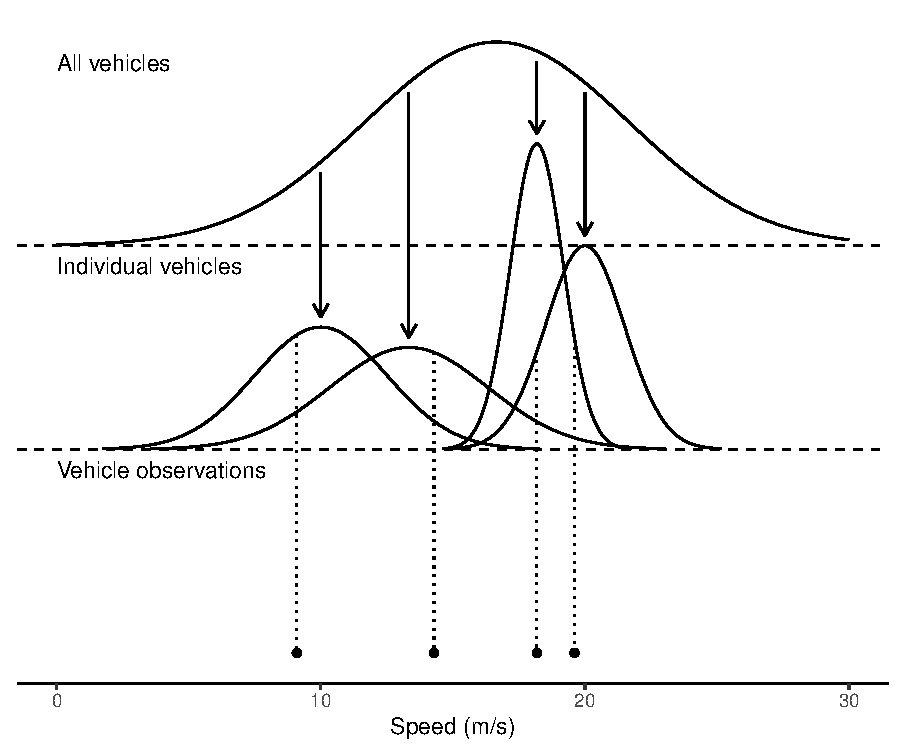
\includegraphics[width=0.6\textwidth]{figure/nw_model_hierarchy-1} 

}

\caption[The hierarchy of speed uncertainty along a single road segment, at one point in time, is separated into \emph{between-vehicle variability} and \emph{measurement error}]{The hierarchy of speed uncertainty along a single road segment, at one point in time, is separated into \emph{between-vehicle variability} and \emph{measurement error}. The top curve shows the underlying distribution of average vehicle speed, with solid arrows showing the true average speed of four vehicles. The second level shows the measurement uncertainty for each vehicle, with the observed values shown as dots at the bottom of the graph.}\label{fig:nw_model_hierarchy}
\end{figure}


\end{knitrout}

\section{A model of average road speed}
\label{sec:nw_model}


The relationship between the underlying road speed and the value observed in \cref{cha:vehicle_model} involves two steps. The first is the relationship between the average traffic speed and the vehicle's true average speed. Second is the relationship between \emph{actual} and \emph{observed} (or, more specifically, estimated) average speed. This type of model is referred to as a \emph{hierarchical (Bayesian) model}, as demonstrated graphically in \cref{fig:nw_model_hierarchy}.


Let us first consider the state of the network at time $t_c$, which we denote
\begin{equation}\label{eq:nw_state}
\boldsymbol{\NWstate}_c =
\left[\NWstate_{1,c}\ \cdots\ \NWstate_{L,c}\right]^\top,
\end{equation}
a vector containing the current real-time average traffic speed along all $L$ roads in the network. However, modelling the full state would increase computational demand as $L$ gets large, so we consider each road segment $\ell$ \emph{independently} (this assumption is revisited in \cref{sec:kf-limits}).


Vehicles travelling along road segment $\ell$ at time $t_c$ have an underlying average speed of $\NWstate_{\ellc}$~seconds, which changes with an average rate of $\NWnoise_\ell$ m/s$^2$. Assuming the underlying road state is a Markov process, the model for the evolution of traffic speed along a road with a maximum velocity (speed) of $\MaxSpeed_\ell$~\gls{mps} is
\begin{equation}\label{eq:nw_state_markov}
\NWstate_{\ellc} \sim
\TNormal{\mathcal{F}_c(\NWstate_{\ellc-1})}{(\NWtdiff_c \NWnoise_c)^2}{0}{\MaxSpeed_\ell},
\end{equation}
where $\NWtdiff_c = t_c - t_{c-1}$ is the time since the last update. This model allows traffic speed to follow temporal trends through the time-dependent transition function $\mathcal{F}_c$ (peak hour traffic, for example) as well as react to real-time events, such as accidents or weather events.


As already mentioned, there are many factors which can affect the speed of a vehicle along a given road segment. To encapsulate this uncertainty, we introduce a single parameter $\NWvar_{\ellc}$, which describes the \emph{between-vehicle variability}, or the width of the distribution at the top of \cref{fig:nw_model_hierarchy}. The true average speed of bus $m$ along road segment $\ell$ at time $t_c$ is denoted $\Vtt_{\ellc}^m$, and is assumed to be an observation from the population distribution with mean $\NWstate_{\ellc}$ and variance $\NWvar_{\ellc}^2$, again truncated appropriately:
\begin{equation}\label{eq:nw_vehicle_tt}
\Vtt_{\ellc}^m \sim
\TNormal{\NWstate_{\ellc}}{\NWvar_{\ellc}^2}{0}{\MaxSpeed_\ell}.
\end{equation}


Once a vehicle has traversed a segment, we estimate its average speed as $\Vttobs_{\ellc}^m$, as estimated in \cref{eq:pf_travel_time_mean} on \cpageref{eq:pf_travel_time_mean}. We assume the measurement is made with uncertainty $\Vtterr_{\ellc}^m$, as demonstrated in \cref{fig:nw_model_hierarchy} as the second level of the hierarchy, which is expressed as
\begin{equation}\label{eq:nw_tt_obs_dist}
\Vttobs_{\ellc}^m \sim \Normal{\Vtt_{\ellc}^m}{(\Vtterr_{\ellc}^m)^2}.
\end{equation}



To assess the model, we performed a simulation where all the parameter values are known (based off of the values estimated in \cref{sec:nw_par_est}). \Cref{fig:nw_sim_data} shows the three stages of the model hierarchy.


\begin{knitrout}\small
\definecolor{shadecolor}{rgb}{0.969, 0.969, 0.969}\color{fgcolor}\begin{figure}

{\centering \subfloat[Underlying average vehicle speed\label{fig:nw_sim_data1}]{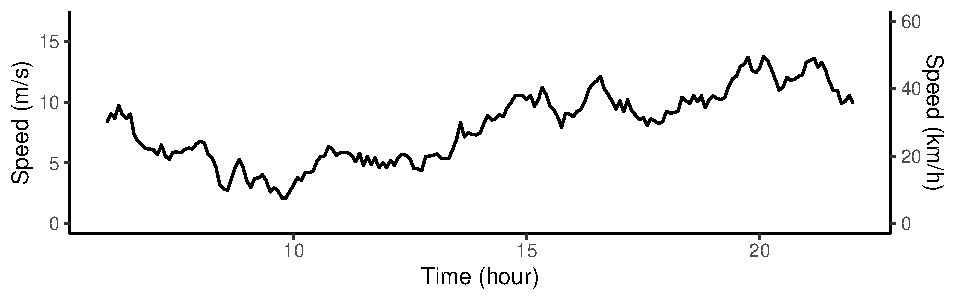
\includegraphics[width=0.8\textwidth]{figure/nw_sim_data-1} }\\
\subfloat[Actual bus speeds (averaged over road segment)\label{fig:nw_sim_data2}]{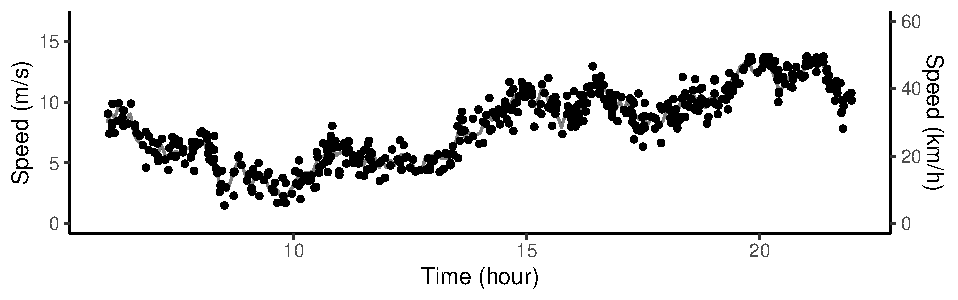
\includegraphics[width=0.8\textwidth]{figure/nw_sim_data-2} }\\
\subfloat[Observed average bus speeds, with vertial lines representing measurement error.\label{fig:nw_sim_data3}]{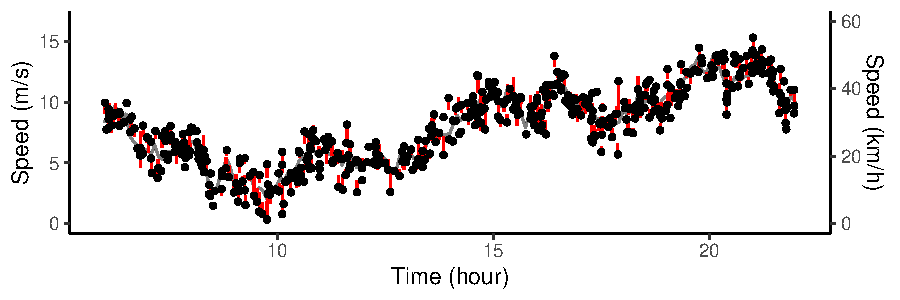
\includegraphics[width=0.8\textwidth]{figure/nw_sim_data-3} }\\

}

\caption[Simulated data showing average vehicle speed along a road]{Simulated data showing average vehicle speed along a road. The right hand axis is shown as a guide for readers not familiar with speeds measured in meters per second.}\label{fig:nw_sim_data}
\end{figure}


\end{knitrout}


Observed vehicle speeds for a real segment, displayed in \cref{fig:tt_figure}, shows some similarities to the simulated data, with one notable difference: the peak-hour spike. This spike is due, in part, to the location of the road, the Symonds Street overbridge:\footnote{Since a lot of traffic arriving into the CBD from the south must use this bridge, it can get very congested.} there is often a (very long) queue of buses from many routes converging there on the central city. In this section, we use the simulated data to evaluate the model under ``nice'' conditions and then test it on this real data to see how well the model copes with these types of phenomenon. The map in \cref{fig:nw_seg_maps} on \cpageref{fig:nw_seg_maps} shows the location of this and several other road segments.


\begin{knitrout}\small
\definecolor{shadecolor}{rgb}{0.969, 0.969, 0.969}\color{fgcolor}\begin{figure}

{\centering 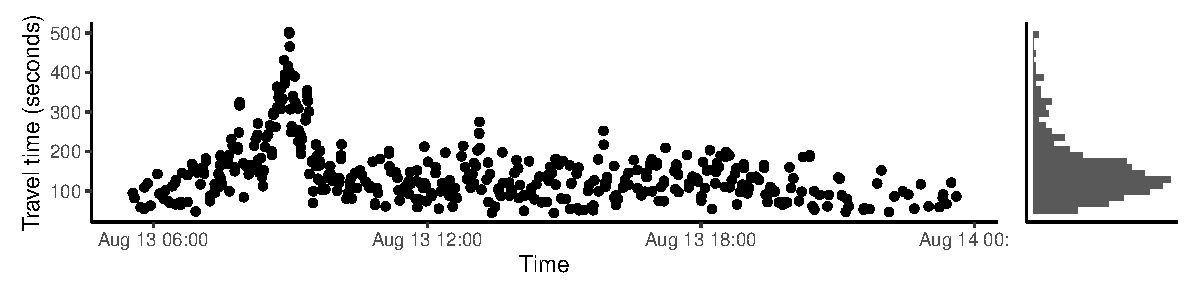
\includegraphics[width=0.8\linewidth]{figure/tt_figure-1} 

}

\caption[Road state observations along a single road segment.]{Road state observations along a single road segment over time, comparing travel time (top) to speed (bottom).}\label{fig:tt_figure}
\end{figure}


\end{knitrout}

\section{Real-time network model}
\label{sec:nw_realtime}

Due to the time constraints of real-time applications, our framework uses a Kalman filter to implement the model described above, which, as previously discussed, is a highly efficient estimation method. This requires the transition and measurement matrices as described in \cref{sec:kf} on \cpageref{sec:kf}. The measurement matrix is the identity matrix $\mat{I}$ since the data are now direct observations of the underlying state (average vehicle speed):
\begin{equation}
\label{eq:kf_meas_identity}
\NWstate_{\ellc} = \mat{H}\Vtt_{\ellc} + w_{\ellc} = \Vtt_{\ellc} + w_{\ellc}
\end{equation}
We also use the identity matrix for the transition matrix $\mat{F}$ as our best guess of the current traffic state is the previous state. So, assuming that $\NWvar_{\ell}$ and $\NWnoise_{\ell}$ are known, for now, we have everything needed to implement a Kalman filter on $\NWstate_{\ellc}$.


\subsection{Predict step}
\label{sec:kf_predict}

In the examples presented, we use a stationary transition function, that is, $\mat{F}_c = 1$, which implies an assumption that traffic speed is constant over short periods (less than five~minutes). The vector of all segment speed observations up to and including time $t_{c}$ is defined as
\begin{equation}\label{eq:all_seg_obs}
\NWobs_{\ell,1:c}^{\boldsymbol{\cdot}} = \bigcup_{t=1}^{c} \bigcup_{v\in V_{\ell,t}} \NWobs_{\ell,t}^v,
\end{equation}
where $V_{\ellc}$ is the set of all vehicles traversing segment $\ell$ at time $t_c$. Then the estimated segment state, conditional on all observations up to time $t_{c-1}$, has mean
\begin{equation}\label{eq:ch4:nw_state_mean_est}
\hat\NWstate_{\ellc|c-1} =
    \E{\NWstate_{\ellc} \cond{} \NWobs_{\ell,1:c-1}^{\boldsymbol{\cdot}}}
\end{equation}
and variance
\begin{equation}\label{eq:ch4:nw_state_var_est}
\NWstatevar_{\ellc|c-1} =
    \Var{\NWstate_{\ellc} \cond{} \NWobs_{\ell,1:c-1}^{\boldsymbol{\cdot}}},
\end{equation}
which are predicted using the following equations:
\begin{equation}
\label{eq:nw_kf_predict}
\begin{split}
\hat\NWstate_{\ellc|c-1} &=
    \hat\NWstate_{
\ellc-1|c-1} \\
\NWstatevar_{\ellc|c-1} &= \NWstatevar_{\ellc-1|c-1} + \left(\NWtdiff_c\NWnoise_\ell\right)^2
\end{split}.
\end{equation}
This prediction is shown in \cref{fig:nw_kf1}. Alternatively, were forecast information available, we could use a transition matrix $\mat F_c$ to describe how traffic might change over time, as is shown in \cref{fig:nw_kf2}.


\begin{knitrout}\small
\definecolor{shadecolor}{rgb}{0.969, 0.969, 0.969}\color{fgcolor}\begin{figure}

{\centering \subfloat[Constant speed model. The prediction is equal to the previous state with an increased variance.\label{fig:nw_kf1}]{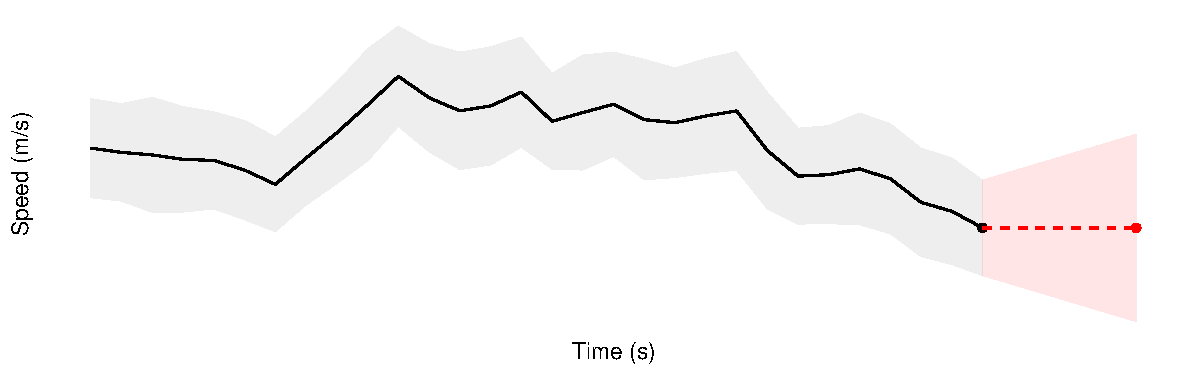
\includegraphics[width=0.8\textwidth]{figure/nw_kf-1} }\\
\subfloat[Historical change based model. The dashed blue line represents historical average speed, which the prediction accounts for under this model.\label{fig:nw_kf2}]{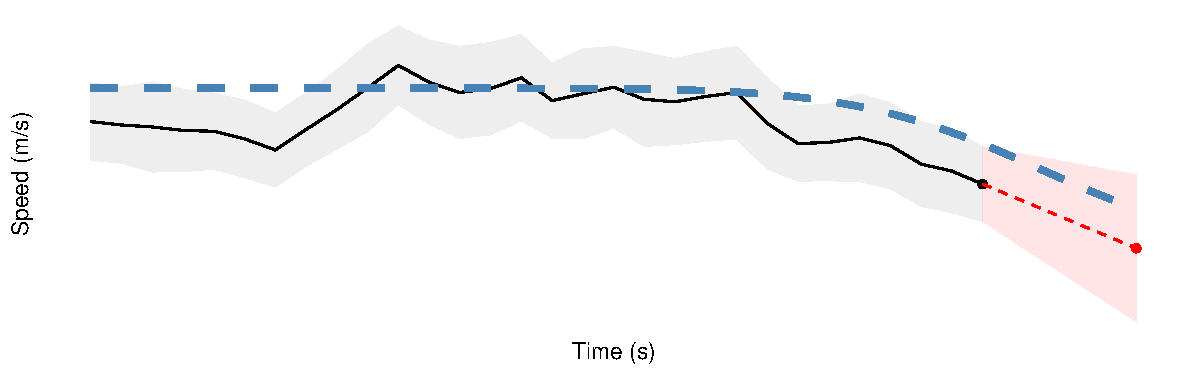
\includegraphics[width=0.8\textwidth]{figure/nw_kf-2} }\\

}

\caption[Network state prediction using constant speed and historical trend models]{Network state prediction depends solely upon the current state (black dot). The mean (solid black line) and uncertainty (shaded grey region) represent previous states. The predicted state has mean (red point) and uncertainty (shared pink region) dependent on the chosen model.}\label{fig:nw_kf}
\end{figure}


\end{knitrout}


\subsection{Update step}
\label{sec:kf_update}

Updating the \kf{} involves taking the predicted state and updating it using \emph{observations} of vehicle speeds along road segments. These are obtained from the \pf{} (\cref{sec:vehicle_speeds}). However, it is possible to have multiple observations per road segment in one update period, as it is common for buses to travel one behind the other, particularly along bus lanes. Therefore, we have a vector of observations passing through segment $\ell$ in the time interval $(t_{c-1}, t_c]$,
\begin{equation} \label{eq:nw_seg_obs}
\NWobss_{\ell c} = \bigcup_{v\in V_{\ell c}} \NWobss_{\ell c}^v,
\end{equation}
which can be the empty set $\NWobss_{\ell c} = \emptyset$ if no vehicles travel through the segment in the interval.


When updating the network, each observation must be accounted for. One way would be to combine the observations into a single estimate; however, this involves averaging observations and uncertainties. An alternative is to use an \emph{\infil{}}, which allows the summation of information from multiple observations \citep{Mutambara_2000}. The information filter involves inverting the state uncertainty $\NWstatevar$; however, this is a simple computation due to having a one-dimensional state---if we were to estimate the state of all segments simultaneously, inverting the $L\times L$ uncertainty matrix would be computationally demanding, or even impossible, and we would be unable to use the approach.



The first step converts the predicted state vector and covariance matrix into information space by inversion of the covariance matrix, leading to the information matrix
\begin{equation}\label{eq:nw_if_inf_matrix}
\NWinfmat_{\ellc|c-1} = \NWstatevar_{\ellc|c-1}^{-1}
\end{equation}
and information vector
\begin{equation}\label{eq:nw_if_inf_vector}
\hat\NWinfvec_{\ellc|c-1} = \NWstatevar_{\ellc|c-1}^{-1} \hat\NWstate_{c|c-1}.
\end{equation}


Converting the observations into information follows the same formula. Note first that the error needs to account for both measurement error and between-vehicle variation, which are assumed Gaussian and independent, so the total variance is their sum. The observation information matrix is
\begin{equation}\label{eq:nw_if_inf_obsmatrix}
\NWobsinfmat_{\ellc}^v = \frac{1}{\NWvar_{\ell}^2 + (\NWerr_{\ellc}^v)^2}
\end{equation}
and the observation information vector is
\begin{equation}\label{eq:nw_if_inf_obsvector}
\hat\NWobsinfvec_{\ellc}^v = \frac{\hat\NWobs_{\ellc}^v}{
    \NWvar_{\ell}^2 + (\NWerr_{\ellc}^v)^2
}.
\end{equation}
Combining these by summation over vehicles yields the complete information matrix and vector for the time period $(t_{c-1},t_c]$, which are, respectively,
\begin{equation}\label{eq:nw_if_obsupdate_matrix}
\NWobsinfmat_{\ellc} = \sum_{v\in V_{\ellc}} \NWobsinfmat_{\ellc}^v
\end{equation}
and
\begin{equation}\label{eq:nw_if_obsupdate_vector}
\NWobsinfvec_{\ellc} = \sum_{v \in V_{\ellc}} \NWobsinfvec_{\ellc}^v.
\end{equation}



The state update is now just a case of adding the observation information in \cref{eq:nw_if_inf_obsmatrix,eq:nw_if_inf_obsvector} to the predicted state information in \cref{eq:nw_if_inf_matrix,eq:nw_if_inf_vector}:
\begin{equation}
\label{eq:nw_if_update}
\begin{split}
\NWinfmat_{\ellc|c} &= \NWinfmat_{\ellc|c-1} + \NWobsinfmat_{\ellc} \\
\hat\NWinfvec_{\ellc|c} &= \hat\NWinfvec_{\ellc|c-1} + \NWobsinfvec_{\ellc}
\end{split}.
\end{equation}
Note that, in situations where no data is observed for a given segment, the information for that segment is zero, so there is no further change to the predicted state value. This could be useful at peak hour, for example, if the transition function predicts changes based on historical trends.


Finally, we back-transform the information into the state space,
\begin{equation}
\label{eq:nw_if_statespace}
\begin{split}
\hat\NWstate_{\ellc|c} &= \NWinfmat_{\ellc|c}^{-1} \hat\NWinfvec_{\ellc|c} \\
\NWstatevar_{\ellc|c} &= \NWinfmat_{\ellc|c}^{-1}
\end{split}.
\end{equation}

The primary constraint on the model is the dependence on $\NWvar_{\ell}$ and $\NWnoise_{\ell}$; however, before considering the estimation of these values, we apply the Kalman filter model to the simulated data in \cref{fig:nw_sim_data} for which the parameter values are known.


\begin{knitrout}\small
\definecolor{shadecolor}{rgb}{0.969, 0.969, 0.969}\color{fgcolor}\begin{figure}

{\centering \subfloat[\kf{} estimate of the state mean (red line) and variance (shaded region) along with the true value (dashed black line).\label{fig:nw_simdata_fit1}]{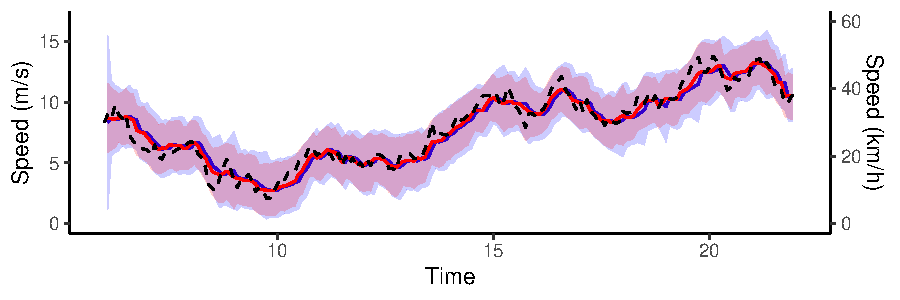
\includegraphics[width=.8\textwidth]{figure/nw_simdata_fit-1} }\\
\subfloat[Predictive distribution of average vehicle speed accounting for state uncertainty and between-vehicle uncertainty ($\NWvar^2$). Observations represented by black points.\label{fig:nw_simdata_fit2}]{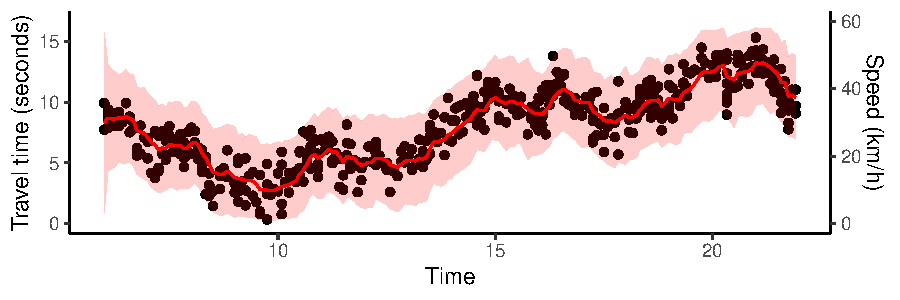
\includegraphics[width=.8\textwidth]{figure/nw_simdata_fit-2} }\\

}

\caption[Results of fitting the \kf{} to the simulated data]{Results of fitting the \kf{} to the simulated data.}\label{fig:nw_simdata_fit}
\end{figure}


\end{knitrout}

The \kf{} was fitted to the simulated data using the same values of $\NWnoise_\ell$ and $\NWvar_\ell$ used to generate the data, with the estimate of $\NWstate_{\ell,1:c}$ shown by the solid red line in \cref{fig:nw_simdata_fit1} along with the associated uncertainty as estimated by $\NWstatevar_{\ell,1:c}$ (shaded region). A dashed black line represents the simulated true mean. We see that the 95\% credible region contains the true values of $\NWstate_{\ell,1:c}$. \Cref{fig:nw_simdata_fit2} shows the posterior estimate of $\NWstate_{\ell,1:c}$ along with the posterior predictive distribution of $\NWobs_{\ellc}^m$; that is, using the 95\% region defined by the sum of $\NWstatevar_{\ell,1:c}$ and $\NWvar_\ell^2$, the latter of which is known for the simulation. 99.8\% of the observations lie within the 95\% predictive region. Given the network parameters $\NWnoise_\ell$ and $\NWvar_\ell$ are known, the underlying network state can be recovered using a \kf{}.


\subsection{Limitations of the implementations}
\label{sec:kf-limits}

The main limitation of using the information filter is the need to calculate the inverse of the covariance matrix. If we want to improve the model by including segment interactions, the dimensionality of $\NWstatevar$ would quickly become too large to compute $\NWstatevar^{-1}$ easily. Thus, the method presented here is only appropriate for independent segments. Fortunately, however, using the \kf{} instead would not be too difficult a task, since most of the time, only one vehicle will pass through a segment during an iteration. In cases where there is more than one, the estimates and their errors could be combined using a sample mean and variance, for example.


\section{Estimating network parameters}
\label{sec:nw_par_est}


To use the \kf{} in any meaningful way, we first need to estimate the system noise, $\NWnoise_\ell$, and the between-vehicle variance, $\NWvar_{\ell}^2$. To estimate values for these parameters, we fit the same model from \cref{sec:nw_model} to the historical data shown in \cref{fig:tt_figure} using \gls{mcmc} sampling methods as implemented by \prog{JAGS} \citep{JAGS}.


The first step in the modelling process fits the following hierarchical model:
\begin{equation}
\label{eq:nw_model_simple}
\begin{split}
\Vttobs_{\ellc}^m \cond \Vtt_{\ellc}^m &\sim \Normal{\Vtt_{\ellc}^m}{(\Vtterr_{\ellc}^m)^2}, \\
\Vtt_{\ellc}^m \cond \NWstate_{\ellc}, \NWvar_{\ell} &\sim \TNormal{\NWstate_{\ellc}}{\NWvar_{\ell}^2}{0}{\MaxSpeed_\ell}, \\
\NWstate_{\ell,0} &\sim \Uniform{0}{\MaxSpeed_\ell}, \\
\NWstate_{\ellc} \cond \NWstate_{\ell-1,c}, \NWnoise_\ell &\sim \TNormal{\NWstate_{\ell-1,c}}{(\NWtdiff_c \NWnoise_{\ell})^2}{0}{\MaxSpeed_\ell}, \\
\NWnoise_\ell &\sim \GammaD{0.01}{0.01}, \\
\NWvar_\ell &\sim \GammaD{0.01}{0.01}.
\end{split}
\end{equation}
The observation error, as in the previous section, is assumed to be constant for all observations, $\Vtterr_{\ellc}^m = 0.8$~\gls{mps} (which is about 10~km/h). The model implementation was performed from \Rstats{} using the \pkg{rjags} package \citep{rjags}. The model output was processed using the \pkg{tidybayes} package \citep{tidybayes} and graphed using \pkg{ggplot2} \citep{ggplot2}. The \pkg{coda} package was used to assess the model's convergence results \citep{coda}.


\subsection{Simulated data}
\label{nw_par_est_sim}

\begin{knitrout}\small
\definecolor{shadecolor}{rgb}{0.969, 0.969, 0.969}\color{fgcolor}\begin{figure}

{\centering 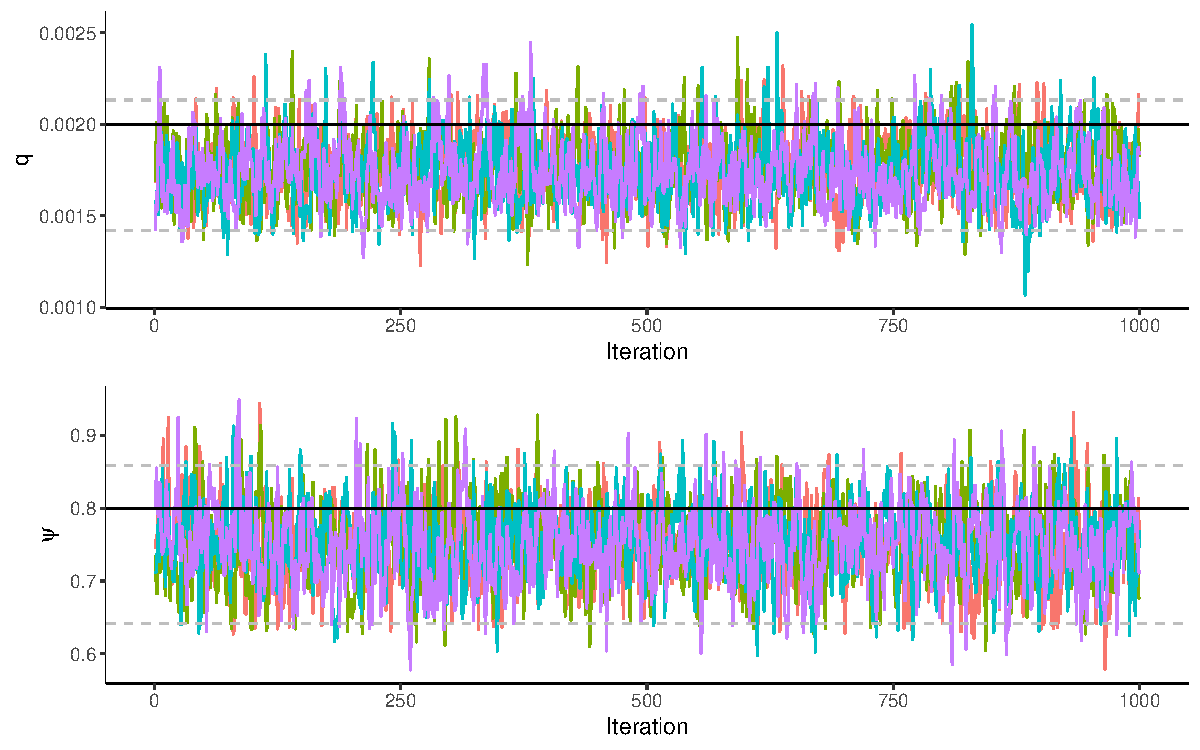
\includegraphics[width=0.8\textwidth]{figure/nw_model_sim_results-1} 

}

\caption[Traceplots of model parameters for the simulated data]{Traceplots of model parameters for the simulated data. Each of the four chains are coloured separately. Dashed grey lines show the 95\% posterior credible interval and the solid lines represent the true values or each parameter.}\label{fig:nw_model_sim_results}
\end{figure}


\end{knitrout}


To assess the model, we start by fitting it to the simulated data (\cref{fig:nw_sim_data}), for which we know the values of $\NWnoise_\ell$ and $\NWvar_\ell$. Trace plots of the model parameters shown in \cref{fig:nw_model_sim_results}, with the true values overlaid with a dashed line, show that the chains mixed well. \Cref{tab:nw_model_sim_smry} gives a summary of the simulation values and their posterior estimates, along with convergence statistics. The 95\% credible intervals for the two parameters contain the true values, so there is nothing to suggest the model is inadequate for modelling the simulated data and estimating the network parameters.


\begin{table}

\caption[MCMC results for the Bayesian model fitted to the simulated travel time data]{\label{tab:nw_model_sim_smry}MCMC results for the Bayesian model fitted to the simulated travel time data. The multivariate $\hat R$, including for all of the $\NWstate$ parameters, was 1.04, indicating that convergence had been achieved after 15,000 iterations.}
\centering
\begin{tabular}[b]{llllllr}
\toprule
Parameter & True Value & Mean & 2.5\% & 50\% & 97.5\% & $\hat R$\\
\midrule
$\NWnoise_\ell$ & 0.002 & 0.0017 & 0.0014 & 0.0017 & 0.0021 & 1.001\\
$\NWvar_\ell$ & 0.8 & 0.75 & 0.64 & 0.75 & 0.86 & 1.001\\
\bottomrule
\end{tabular}
\end{table}





\subsection{Real data}
\label{nw_par_est_real}



Having shown that the \prog{JAGS} model is a valid way of estimating the network parameters $\NWnoise_\ell$ and $\NWvar_\ell$, we model the real travel time data from \cref{fig:tt_figure}. Trace plots of the network parameters, as shown in \cref{fig:nw_model_n1_view}, show again that the chains mixed well, which is reaffirmed by the convergence results in \cref{tab:nw_model_fit_smry}. Not shown here are the summaries of the $\NWstate$'s (there are 187 of them); however, the Gelman diagnostic $\hat R$ was less than 1.03 for all of them, indicating they reached convergence.

\begin{knitrout}\small
\definecolor{shadecolor}{rgb}{0.969, 0.969, 0.969}\color{fgcolor}\begin{figure}

{\centering 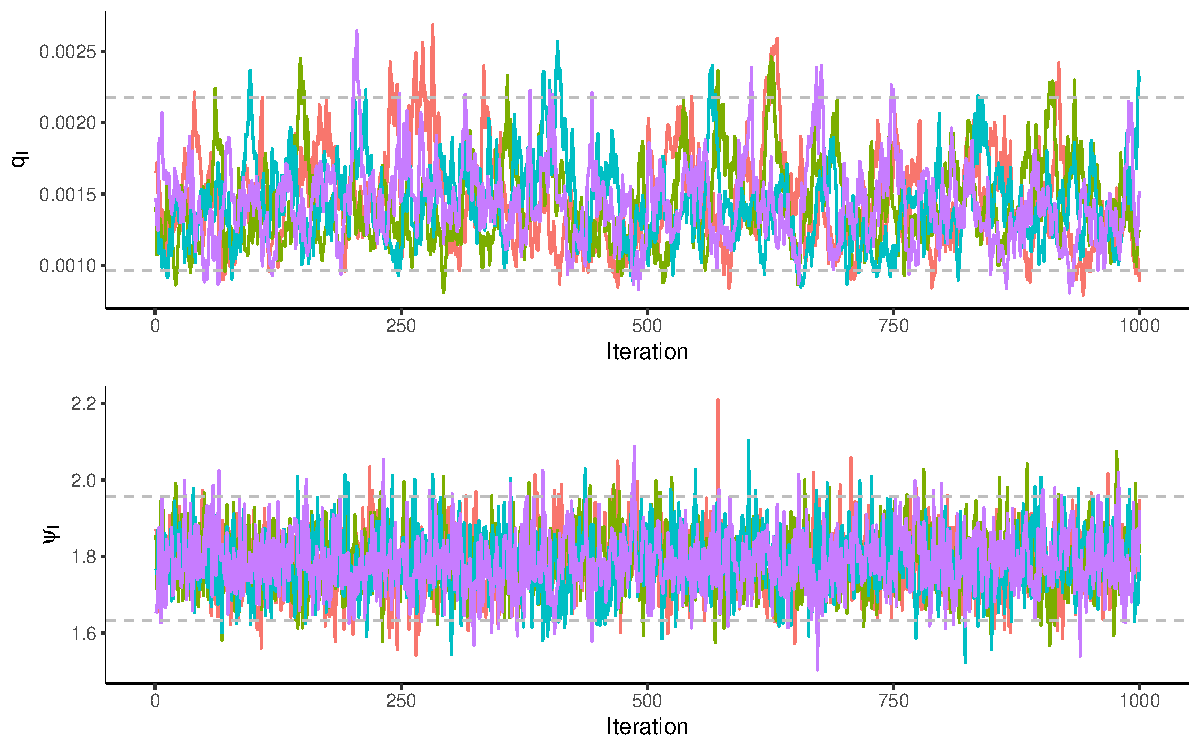
\includegraphics[width=0.8\linewidth]{figure/nw_model_n1_view-1} 

}

\caption[Traceplots of model parameters fitted to the segment data]{Traceplots of model parameters $\NWnoise$ and $\NWvar$ fitted to the segment data. Each of the four chains are coloured separately. The 95\% posterior credible region is denoted by dashed grey lines.}\label{fig:nw_model_n1_view}
\end{figure}


\end{knitrout}

\begin{table}

\caption[MCMC results for the Bayesian model fitted to the road segment travel time data]{\label{tab:nw_model_fit_smry}MCMC results for the Bayesian model fitted to the road segment travel time data. The multivariate $\hat R$, including for all of the $\NWstate$ parameters, was 1.08, indicating that convergence had been achieved after 15,000 iterations.}
\centering
\begin{tabular}[b]{lllllr}
\toprule
Parameter & Mean & 2.5\% & 50\% & 97.5\% & $\hat R$\\
\midrule
$\NWnoise_\ell$ & 0.0015 & 0.001 & 0.0015 & 0.0022 & 1.013\\
$\NWvar_\ell$ & 1.94 & 1.8 & 1.94 & 2.1 & 1.002\\
\bottomrule
\end{tabular}
\end{table}



To assess the adequacy of these parameters, we fit the \kf{} to the same data\footnote{In the next section we use two weeks of data, one for each of testing and training.} to see how well the mean and predictive distributions fit the data. The estimates of $\NWstate_{\ell,1:c}$, along with associated uncertainties, are shown in \cref{fig:nw_model_n1_kf1}, where we see that the mean approximately follows the center of the data. The predictive vehicle speed distribution, which accounts for both $\NWstatevar_{\ell,1:c}$ and between-vehicle uncertainty, $\NWvar_{\ell}$, is shown in \cref{fig:nw_model_n1_kf2}, and shows most of the points contained within the 95\% posterior predictive region.


\begin{knitrout}\small
\definecolor{shadecolor}{rgb}{0.969, 0.969, 0.969}\color{fgcolor}\begin{figure}

{\centering \subfloat[Estimated mean speed, showing state estimates along with the 95\% credible region.\label{fig:nw_model_n1_kf1}]{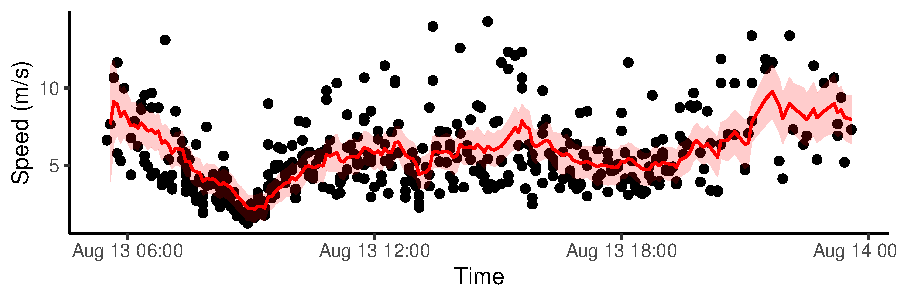
\includegraphics[width=.8\textwidth]{figure/nw_model_n1_kf-1} }\\
\subfloat[Predictive distribution of vehicle speeds, which includes between-vehicle variability.\label{fig:nw_model_n1_kf2}]{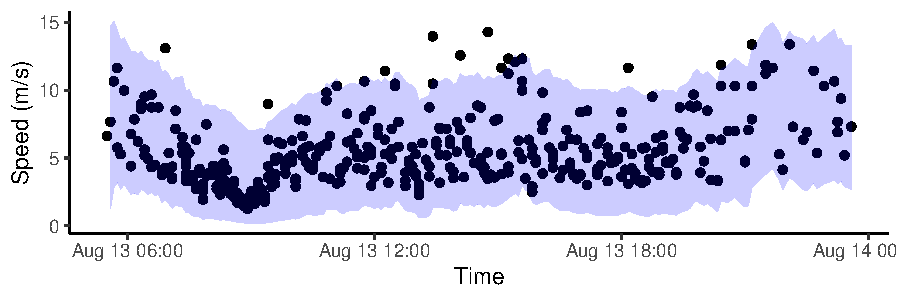
\includegraphics[width=.8\textwidth]{figure/nw_model_n1_kf-2} }\\

}

\caption[Results of fitting a \kf{} to the segment data with parameters estimated using the hierarchical model]{Results of fitting a \kf{} to the segment data with parameters estimated using the hierarchical model.}\label{fig:nw_model_n1_kf}
\end{figure}


\end{knitrout}



Finally, the timing comparison is displayed in \cref{tab:nw_model_n1_timecomp}. The hierarchical model fit using \prog{JAGS} took about 2200 times as long as the \kf{} implementation. So, even if we reduced the number of chains, the number of iterations, and tried to speed up the \prog{JAGS} model, the \kf{} would still be significantly faster.


\begin{table}

\caption[Comparison of the timings for the MCMC and \kf{} estimation methods]{\label{tab:nw_model_n1_timecomp}Comparison of the timings for the MCMC and \kf{} estimation methods. Times are reported in seconds.}
\centering
\begin{tabular}[b]{lrrr}
\toprule
  & User & System & Total\\
\midrule
JAGS & 124.828 & 0 & 124.847\\
Kalman filter & 0.052 & 0 & 0.056\\
\bottomrule
\end{tabular}
\end{table}




\subsection{Hierarchical model over multiple road segments}
\label{sec:nw_par_est_multiple}



To assess how effective our approach is for estimating $\NWvar_\ell$ and $\NWnoise_\ell$, we selected five other road segments around Auckland. However, instead of fitting the same model independently to each segment,  we use a hierarchical Bayesian model on the parameters, since it seems reasonable that, while they will not be the same for all segments, there will be an underlying population distribution. This allows us to obtain estimates of the parameter values without explicitly needing to model every road (of which there are 8,151).


The hierarchical model used to estimate the network parameters is:
\begin{equation}
\label{eq:tt_hist_hier}
\begin{split}
\Vttobs_{\ellc}^m \cond \Vtt_{\ellc}^m &\sim \Normal{\Vtt_{\ellc}^m}{\left(\Vtterr_{\ellc}^m\right)^2}, \\
\Vtt_{\ellc}^m \cond \NWstate_{\ellc}, \NWvar_{\ell} &\sim \TNormal{\NWstate_{\ellc}}{\NWvar_{\ell}^2}{0}{\MaxSpeed_\ell}, \\
\NWstate_{\ell0} &\sim \Normal{0}{10^2}, \\
\NWstate_{\ellc} \cond \NWstate_{\ellc-1}, \NWnoise_{\ell} &\sim \TNormal{\NWstate_{\ellc-1}}{(\NWtdiff_c \NWnoise_{\ell})^2}{0}{\MaxSpeed_\ell}, \\
q &\sim \GammaD{0.001}{0.001}, \\
\log\left(\NWvar_{\ell}\right) \cond \mu_\psi, \sigma_\psi &\sim \Normal{\mu_\psi}{\sigma_\psi^2}, \\
\mu_\psi &\sim \Normal{0}{10^2}, \\
\sigma_\psi &\sim \GammaD{0.001}{0.001}.
\end{split}
\end{equation}
We initially attempted to fit a hierarchical segment noise parameter $\NWnoise_{\ell}$ with hyper\-parameters, but the values were all approximately equal for all segments and convergence was very slow (100,000's of iterations). Instead, we opted for a single common system noise parameter across all segments. The speed data for six segments on two consecutive Tuesdays is shown in \cref{fig:nw_model_n2_segplots}, with the locations of the roads displayed in \cref{fig:nw_seg_maps}.

\begin{knitrout}\small
\definecolor{shadecolor}{rgb}{0.969, 0.969, 0.969}\color{fgcolor}\begin{figure}

{\centering 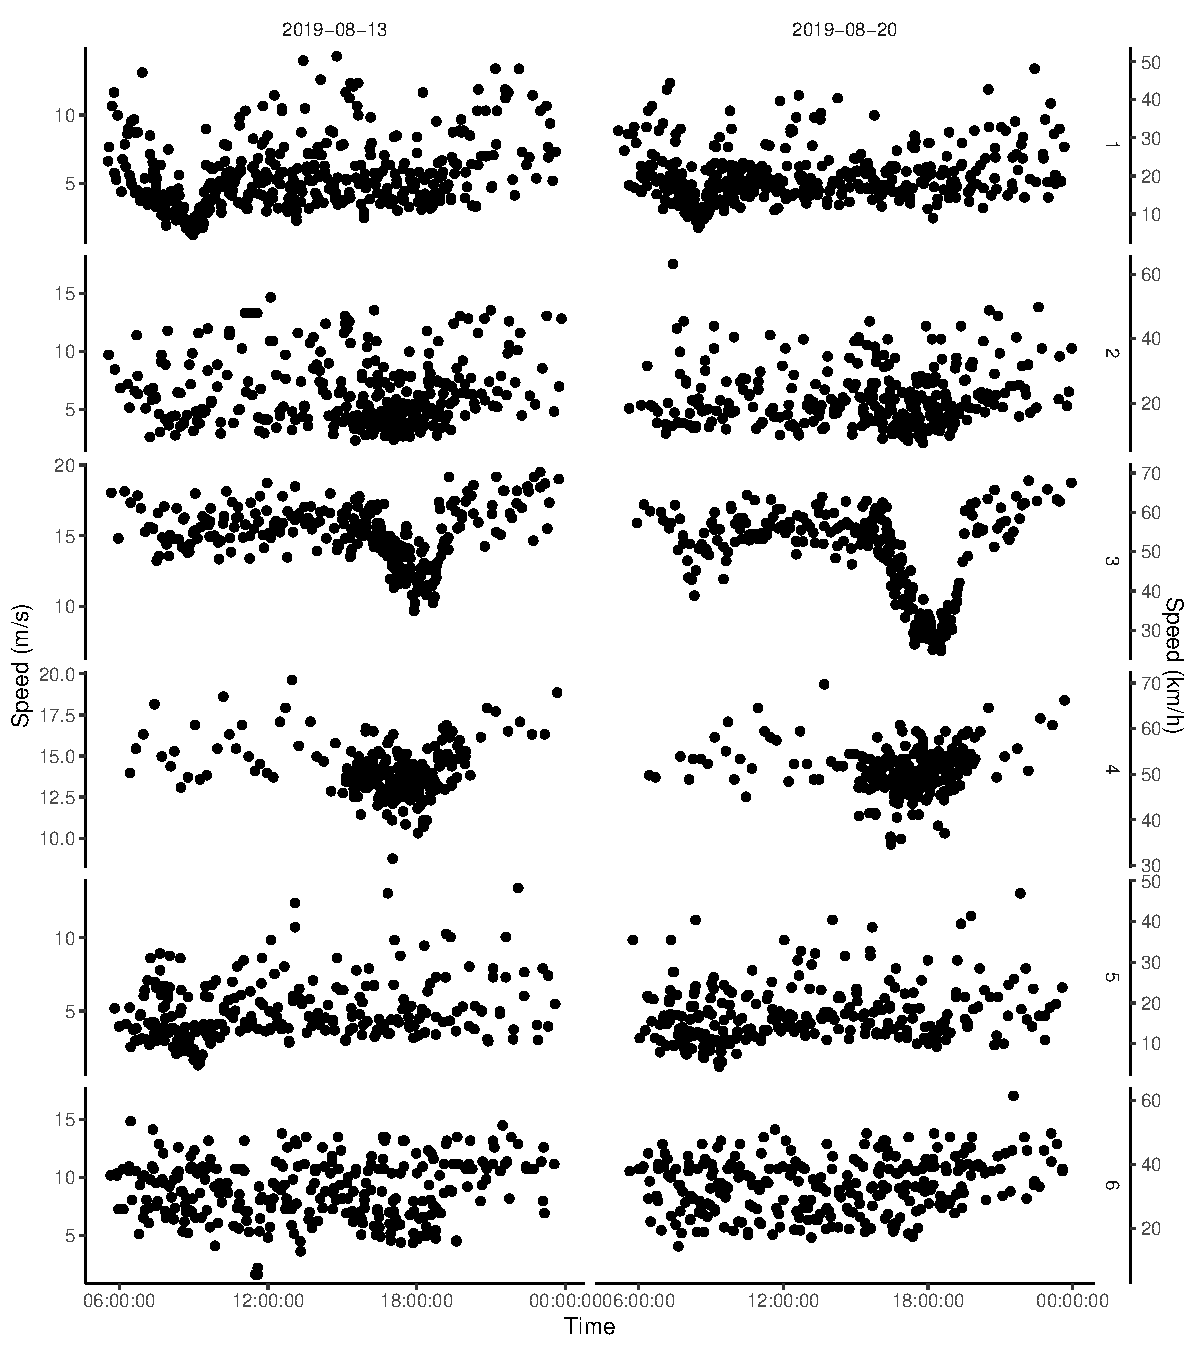
\includegraphics[width=\textwidth]{figure/nw_model_n2_segplots-1} 

}

\caption[Observed average bus speeds along six road segments on two consecutive Tuesdays]{Observed average bus speeds along six road segments on two consecutive Tuesdays.}\label{fig:nw_model_n2_segplots}
\end{figure}


\end{knitrout}

\begin{knitrout}\small
\definecolor{shadecolor}{rgb}{0.969, 0.969, 0.969}\color{fgcolor}\begin{figure}

{\centering 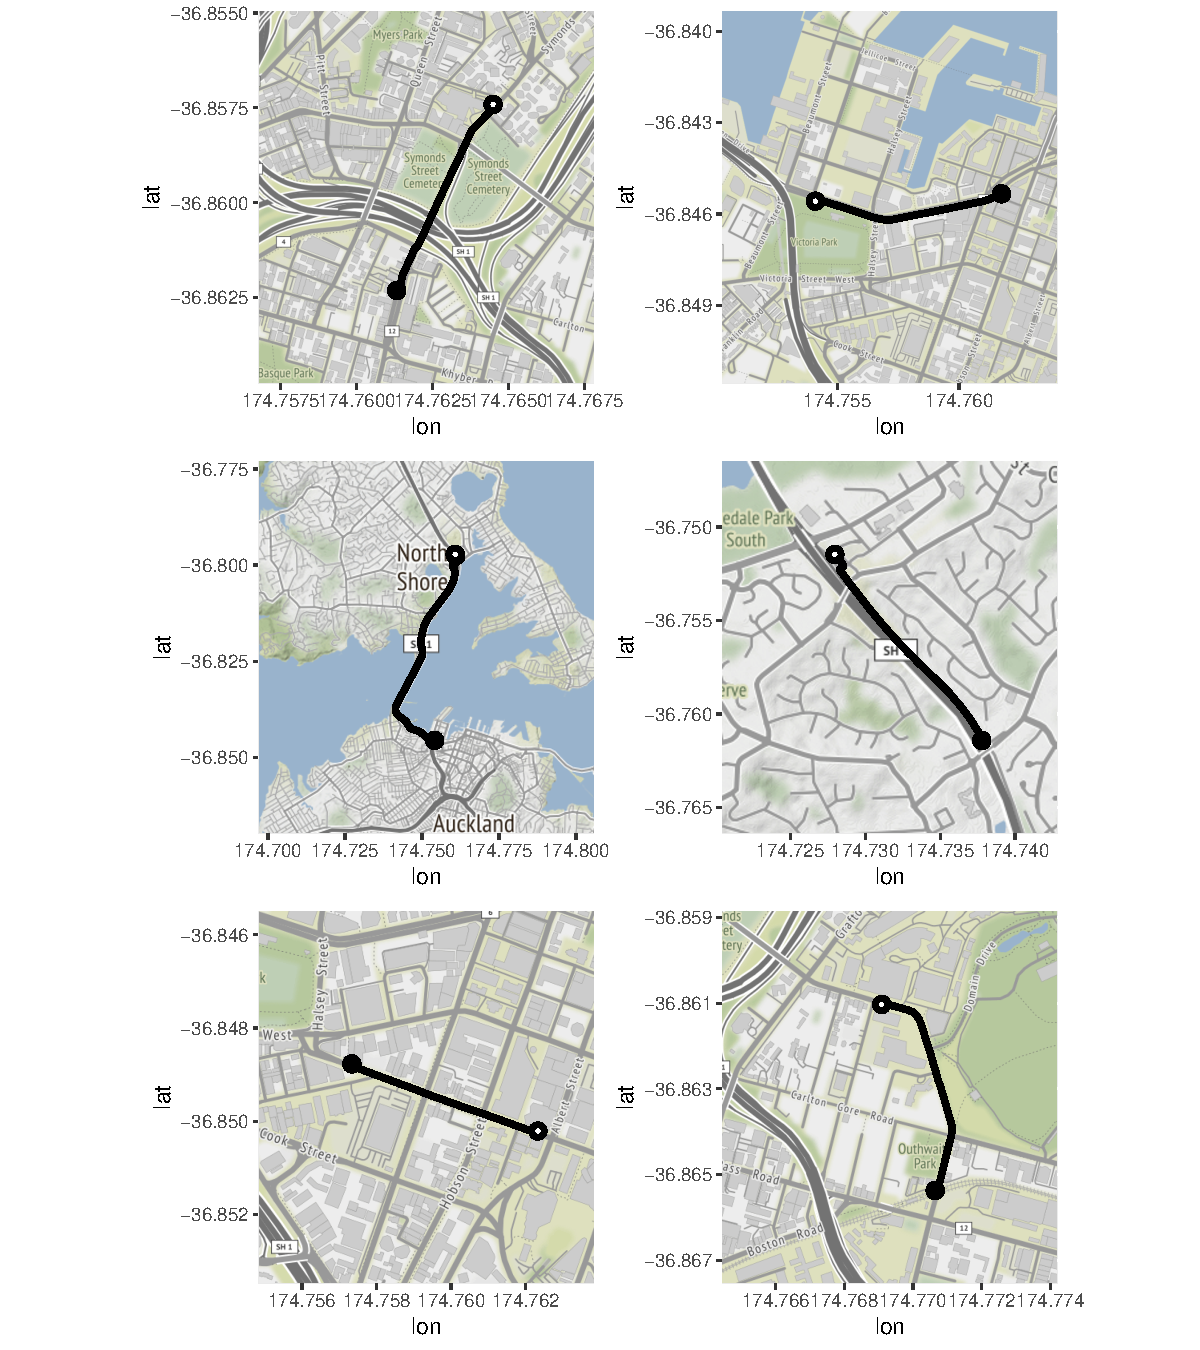
\includegraphics[width=\textwidth]{figure/nw_seg_maps-1} 

}

\caption[Segment locations, drawn using the \pkg{ggmap} package \citep{ggmap}]{Segment locations, drawn using the \pkg{ggmap} package \citep{ggmap}. Segments begin at the solid point and terminate at the open point.}\label{fig:nw_seg_maps}
\end{figure}


\end{knitrout}




\begin{knitrout}\small
\definecolor{shadecolor}{rgb}{0.969, 0.969, 0.969}\color{fgcolor}\begin{figure}

{\centering 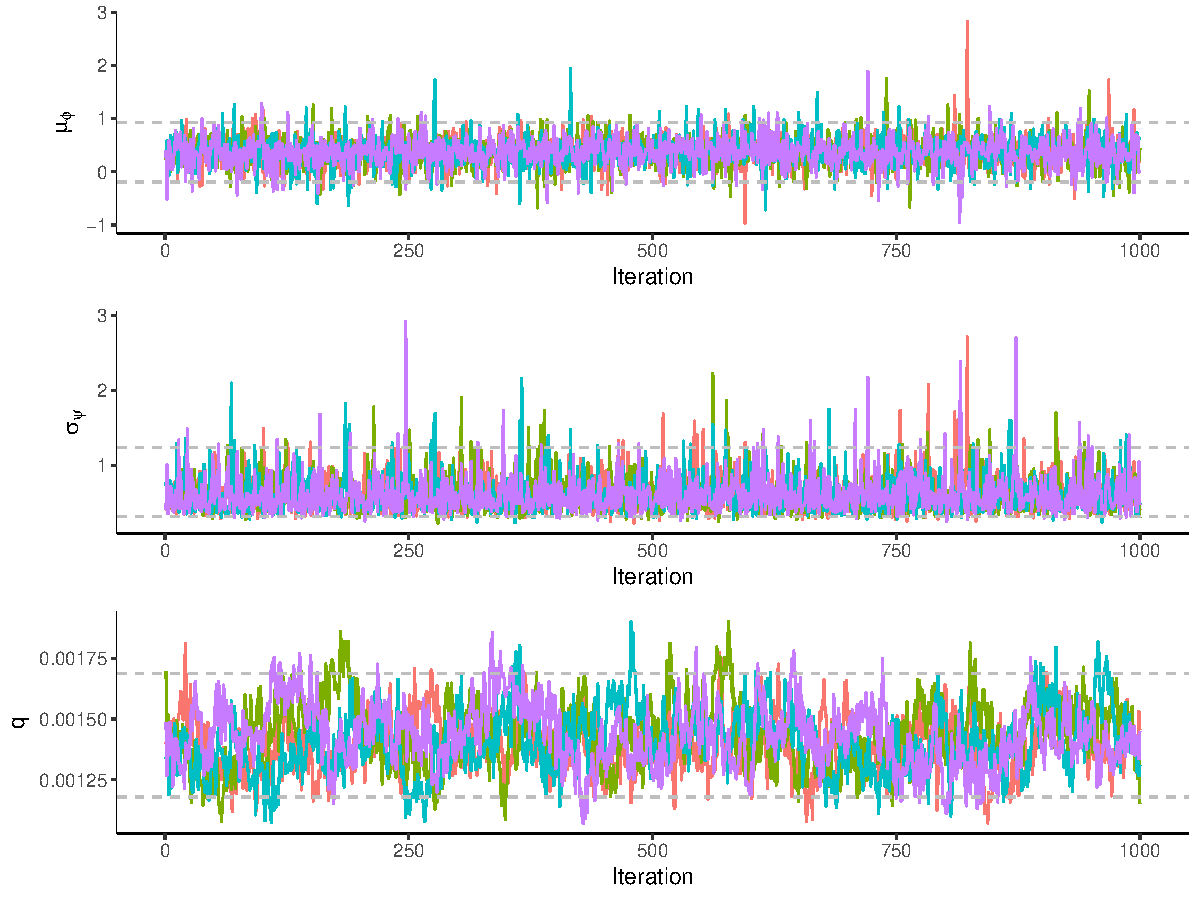
\includegraphics[width=\textwidth]{figure/nw_model_n2_diag-1} 

}

\caption[Traceplots of top-level network parameters estimated by the hierarhical model]{Traceplots of top-level network parameters estimated by the hierarhical model. The four chains are coloured individually, and 95\% credible interval indicated by dashed gray lines.}\label{fig:nw_model_n2_diag}
\end{figure}


\end{knitrout}


\begin{table}

\caption[MCMC results for the hierarchical Bayesian model fitted to six road segments to estimate the top-level variance parameters]{\label{tab:nw_model_n2_smry}MCMC results for the hierarchical Bayesian model fitted to six road segments to estimate the top-level variance parameters. The multivariate $\hat R$, including for all of the $\NWstate$ parameters, was 2.03.}
\centering
\begin{tabular}[b]{lllllr}
\toprule
Parameter & Mean & 2.5\% & 50\% & 97.5\% & $\hat R$\\
\midrule
$\mu_\psi$ & 0.383 & -0.191 & 0.389 & 0.926 & 1.00\\
$\sigma_\psi$ & 0.608 & 0.315 & 0.549 & 1.24 & 1.00\\
$q$ & 0.0014 & 0.0012 & 0.0014 & 0.0017 & 1.02\\
\bottomrule
\end{tabular}
\end{table}




The model was fit using \prog{JAGS} to the first day of data for the six segments, while the second was reserved for testing the validity of the estimated parameters. Each of the four chains was run with a 100,000~iteration burn-in phase, followed by 50,000 iterations with a thinning interval of 50. Trace plots of the top-level parameters are displayed in \cref{fig:nw_model_n2_diag}, which demonstrates good mixing of the chains. \Cref{tab:nw_model_n2_smry} shows the posterior mean and quantiles for these parameters, along with their Gelman convergence diagnostics.


Trace plots for the segment-specific variance parameters are shown in \cref{fig:nw_model_n2_diag_2}, and also demonstrate good mixing. The Gelman convergence diagnostic is again very close to unity, indicating that running the chain for longer would not decrease the posterior variance by much.



\begin{knitrout}\small
\definecolor{shadecolor}{rgb}{0.969, 0.969, 0.969}\color{fgcolor}\begin{figure}

{\centering 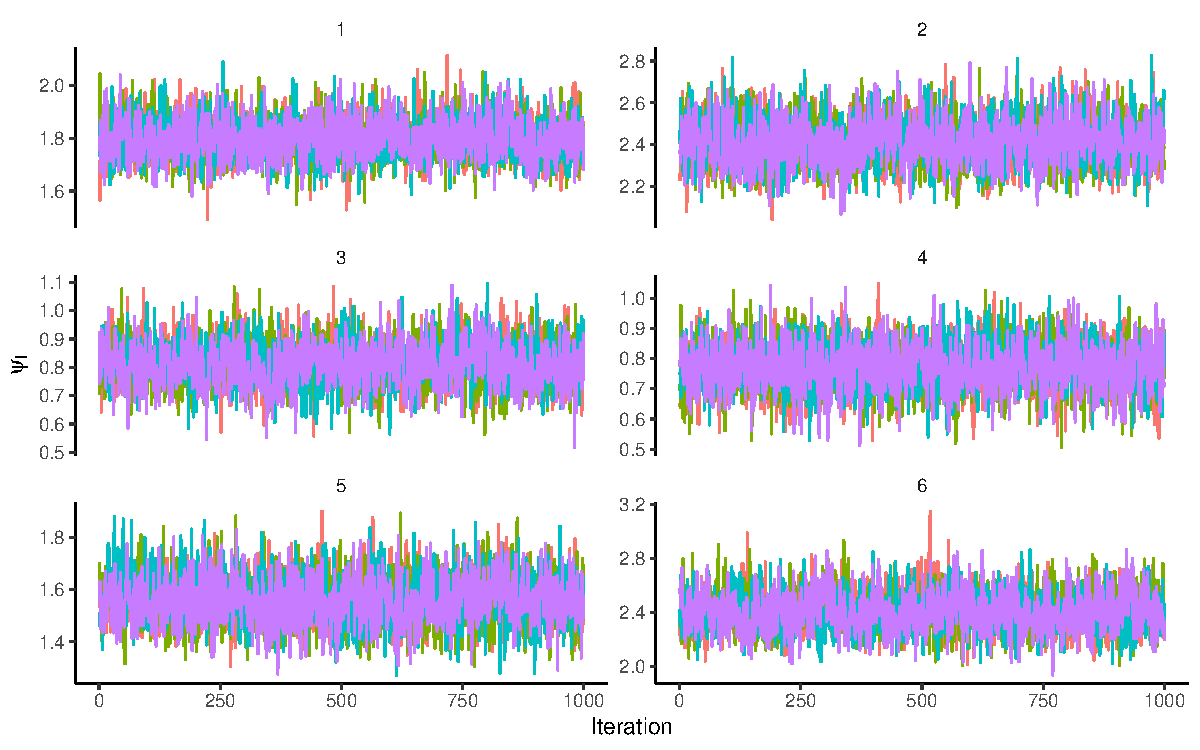
\includegraphics[width=\textwidth]{figure/nw_model_n2_diag_2-1} 

}

\caption[Traceplots of between-vehicle variance parameters, $\NWvar_\ell$, for each segment]{Traceplots of between-vehicle variance parameters, $\NWvar_\ell$, for each segment. The four chains are coloured individually.}\label{fig:nw_model_n2_diag_2}
\end{figure}


\end{knitrout}


The \kf{} was fit to each segment using the posterior mean of $\NWvar_\ell$ and the population parameters. \Cref{fig:nw_model_n2_kf} shows the original data superimposed with a posterior sample of $\NWstate$'s, along with the next week's data with results from the \kf{}, including the 95\% credible region for the mean road speed and the 95\% posterior predictive region for individual vehicles' average speeds.







\begin{knitrout}\small
\definecolor{shadecolor}{rgb}{0.969, 0.969, 0.969}\color{fgcolor}\begin{figure}
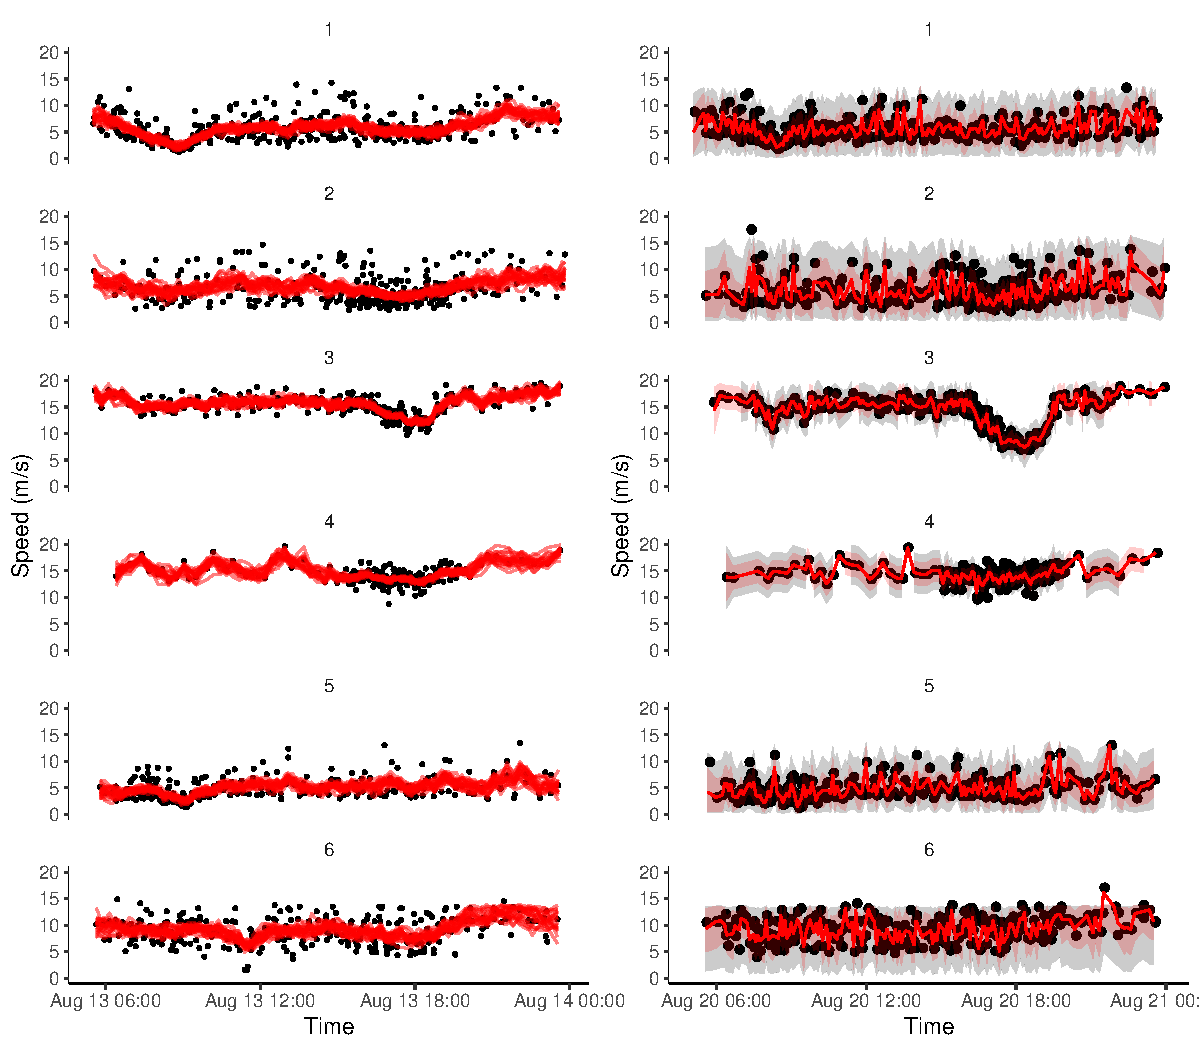
\includegraphics[width=\textwidth]{figure/nw_model_n2_kf-1} \caption[Results for the hierarchical approach to modelling road speed]{Results for the hierarchical approach to modelling road speed. Left: the training data with a sample of posterior fits for \prog{JAGS}. Right: the test data with the Kalman filter estimation results, showing the speed estimate (red line), its uncertainty (shaded in red), and the posterior predictive region for vehicle speeds (shaded in grey).}\label{fig:nw_model_n2_kf}
\end{figure}


\end{knitrout}

The results show that the $\NWstate$ values estimated with \prog{JAGS} nicely fit the data, including peak congestion, as do the \kf{} estimates. The posterior predictive region covers most of the observations for all the segments.

\section{Improving forecasts with history}
\label{sec:nw_hist_model}

The model presented in \cref{sec:nw_model,sec:nw_realtime,sec:nw_par_est} is adequate for estimating the \emph{real-time} state of the network, but is unuseful for forecasting vehicle speeds, particularly just before or after a peak period. In \cref{cha:prediction}, we explore the prediction of arrival times, which involves making short-term forecasts of speed. Using historical data is one way of improving speed forecasts, particularly around peak times.


In \cref{nw_par_est_real}, I showed that most roads have a ``peak effect'' in the morning or the evening, while some exhibit both. It seems reasonable therefore to have a model which allows a segment to have zero, one, or two peaks, each with varying magnitude (the size of the decrease in speed) and width (how long the peak period is). The temporal location of these peaks is likely to be related, but variable: some roads will experience peak traffic earlier than others, for example.

\begin{knitrout}\small
\definecolor{shadecolor}{rgb}{0.969, 0.969, 0.969}\color{fgcolor}\begin{figure}

{\centering 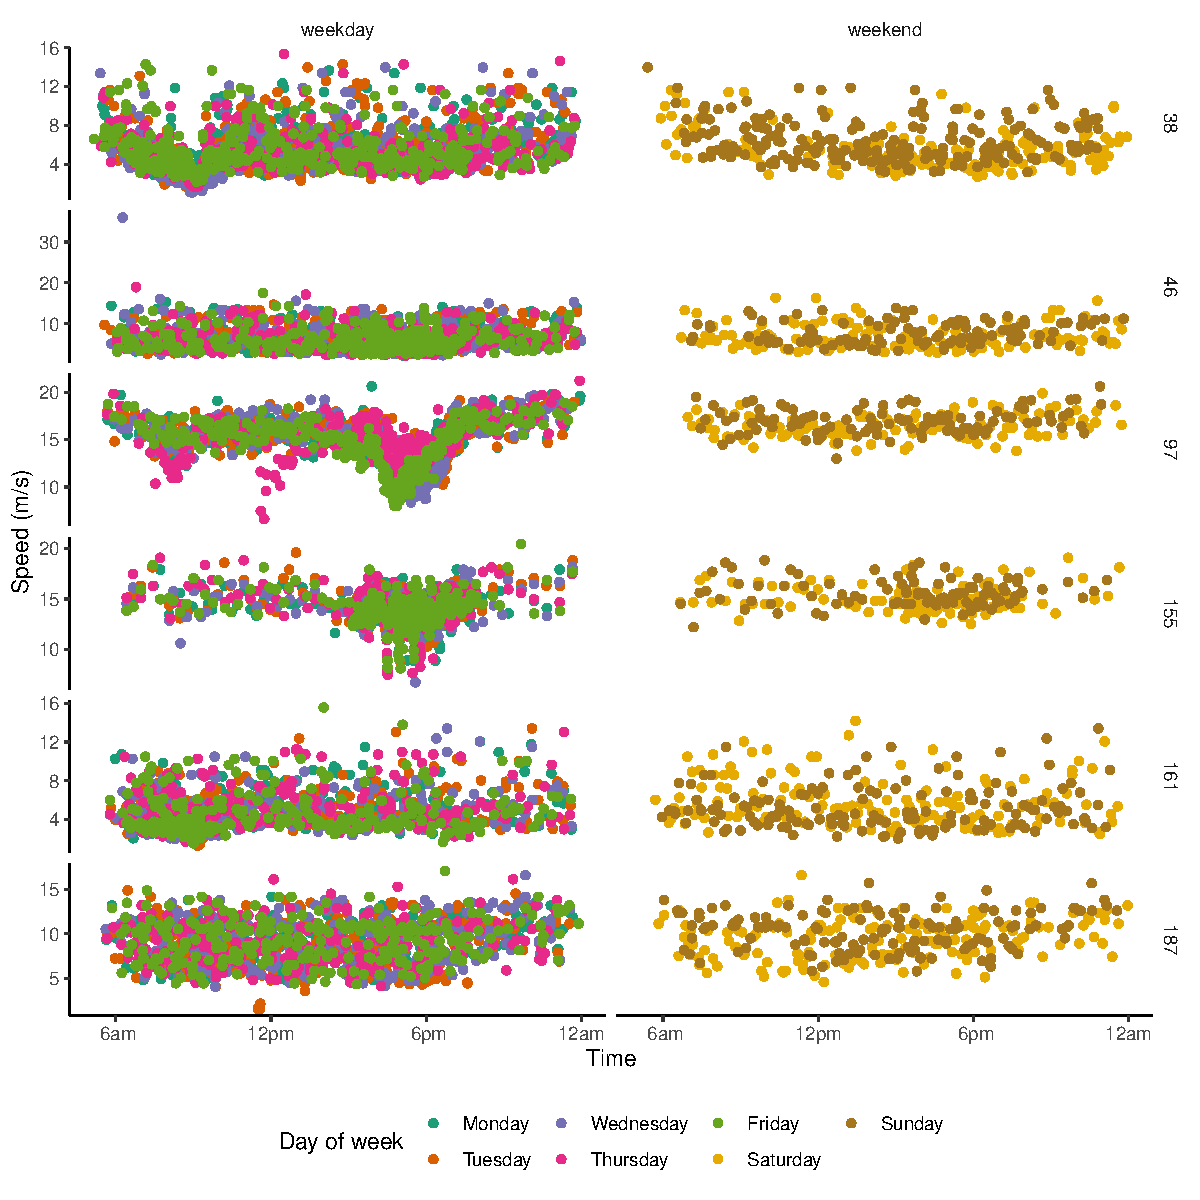
\includegraphics[width=\textwidth]{figure/tt_week0_load-1} 

}

\caption[Vehicle speeds along six road segments over one week]{Vehicle speeds along six road segments over one week, coloured by the day of the week.}\label{fig:tt_week0_load}
\end{figure}


\end{knitrout}

Early work fitting Bayesian models to these data were not promising, as it involved too much manual work tuning the parameters for each segment and checking the results. Since our goal is to obtain a generalised framework that runs with minimal manual effort, we sought an alternative.

From \cref{fig:tt_week0_load} it is clear that along each segment, there is a consistent pattern, with some variability between days as far as the temporal location and magnitude of the ``peak'' on weekdays; weekends are fairly consistent, although this is only two days' worth of data. Here I present a nearest-neighbour grid, which takes time and road state (traffic speed) as input, and outputs the mean (and uncertainty) of travel time in 10, 20, or 30~minutes from the current time. Similar ``speed maps'' have been used by the likes of \citet{Cathey_2003, Celan_2017, Chen_2014}. The first step is to aggregate observations into 5~minute intervals and take the mean traffic speed in each interval. Next, we bind lagged duplicates of these speeds (10, 20, 30~minutes, for example), such that each row includes current and future states. Any missing periods are interpolated from the mean of the adjacent states. The speed map for 30~minute predictions is shown in \cref{fig:tt_week0_grid}. The lighter areas represent higher speeds.







\begin{knitrout}\small
\definecolor{shadecolor}{rgb}{0.969, 0.969, 0.969}\color{fgcolor}\begin{figure}

{\centering 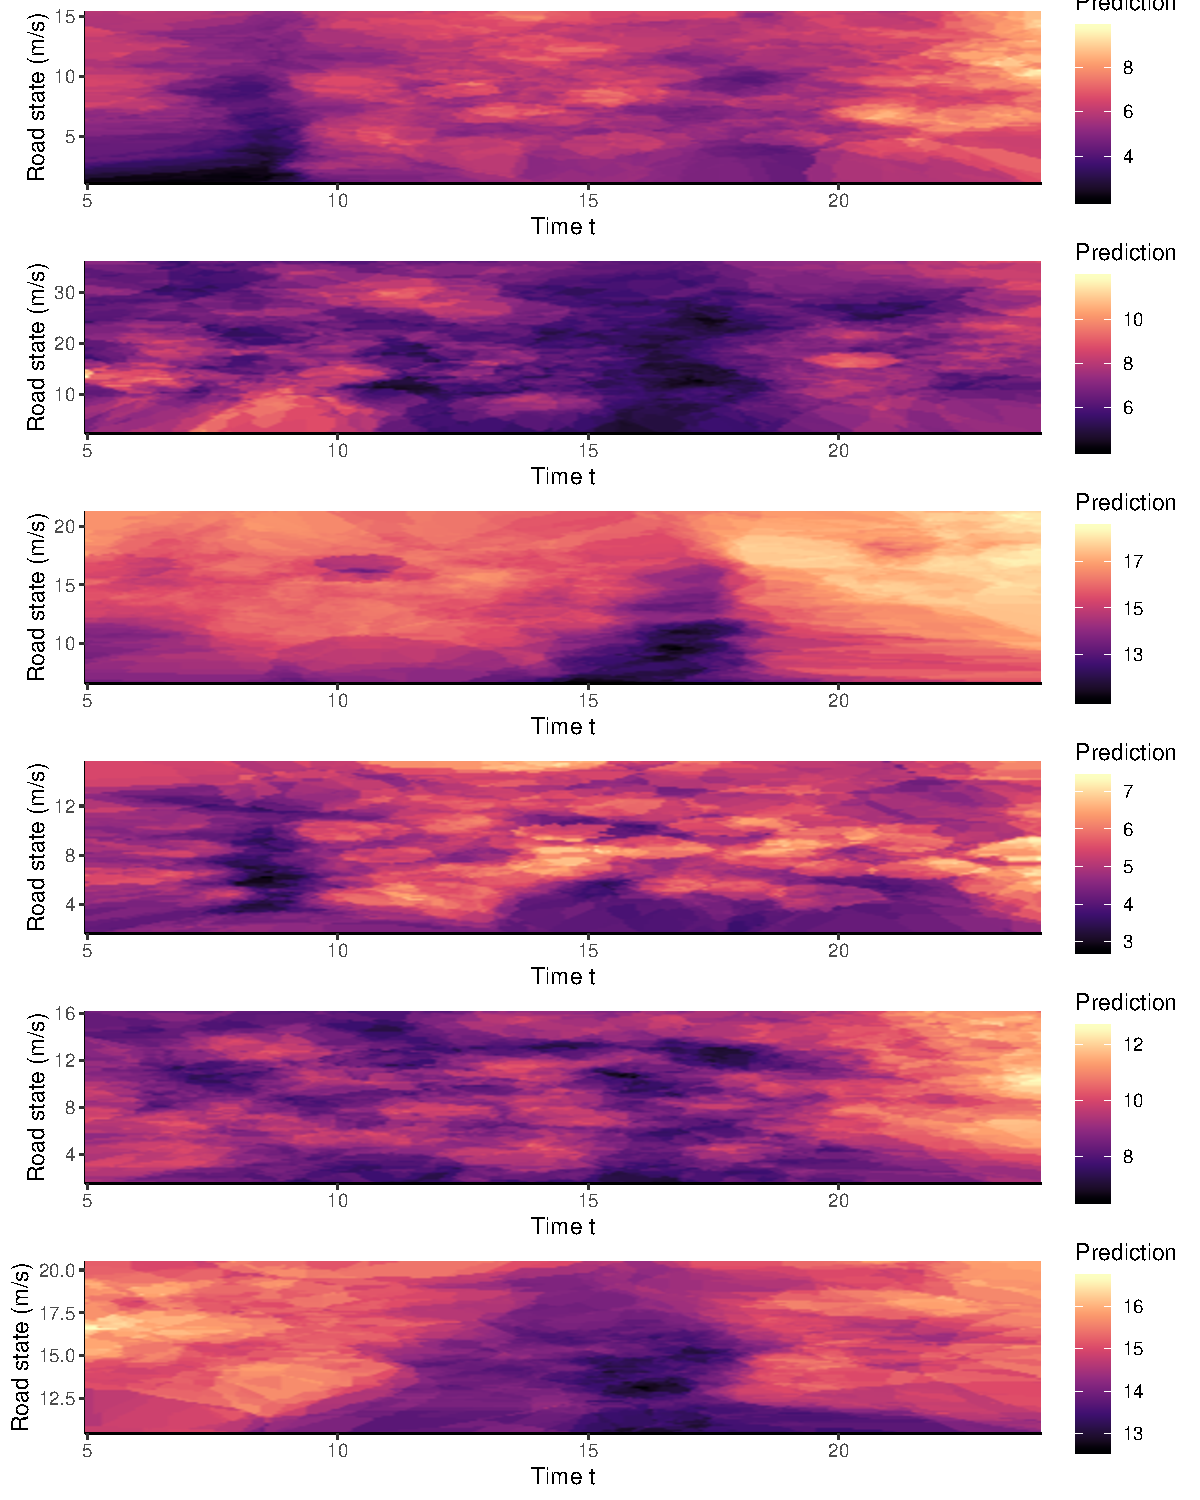
\includegraphics[width=\linewidth]{figure/tt_week0_grid-1} 

}

\caption[Speed maps to predict segment speed in 30~minutes given the current state]{Speed maps to predict segment speed in 30~minutes given the current average speed (y-axis) and time (x-axis).}\label{fig:tt_week0_grid}
\end{figure}


\end{knitrout}

The next step is to evaluate the predictive power of this approach. We do this by taking the second week of data (shown in \cref{fig:tt_week1_load}) and use the fitted estimates to predict the state in 30~minutes, and then compare this to the actual state in 30~minutes. The \gls{rmse} (\cref{app:error-functions}) is used to compare the predicted and observed speeds.



\begin{knitrout}\small
\definecolor{shadecolor}{rgb}{0.969, 0.969, 0.969}\color{fgcolor}\begin{figure}

{\centering 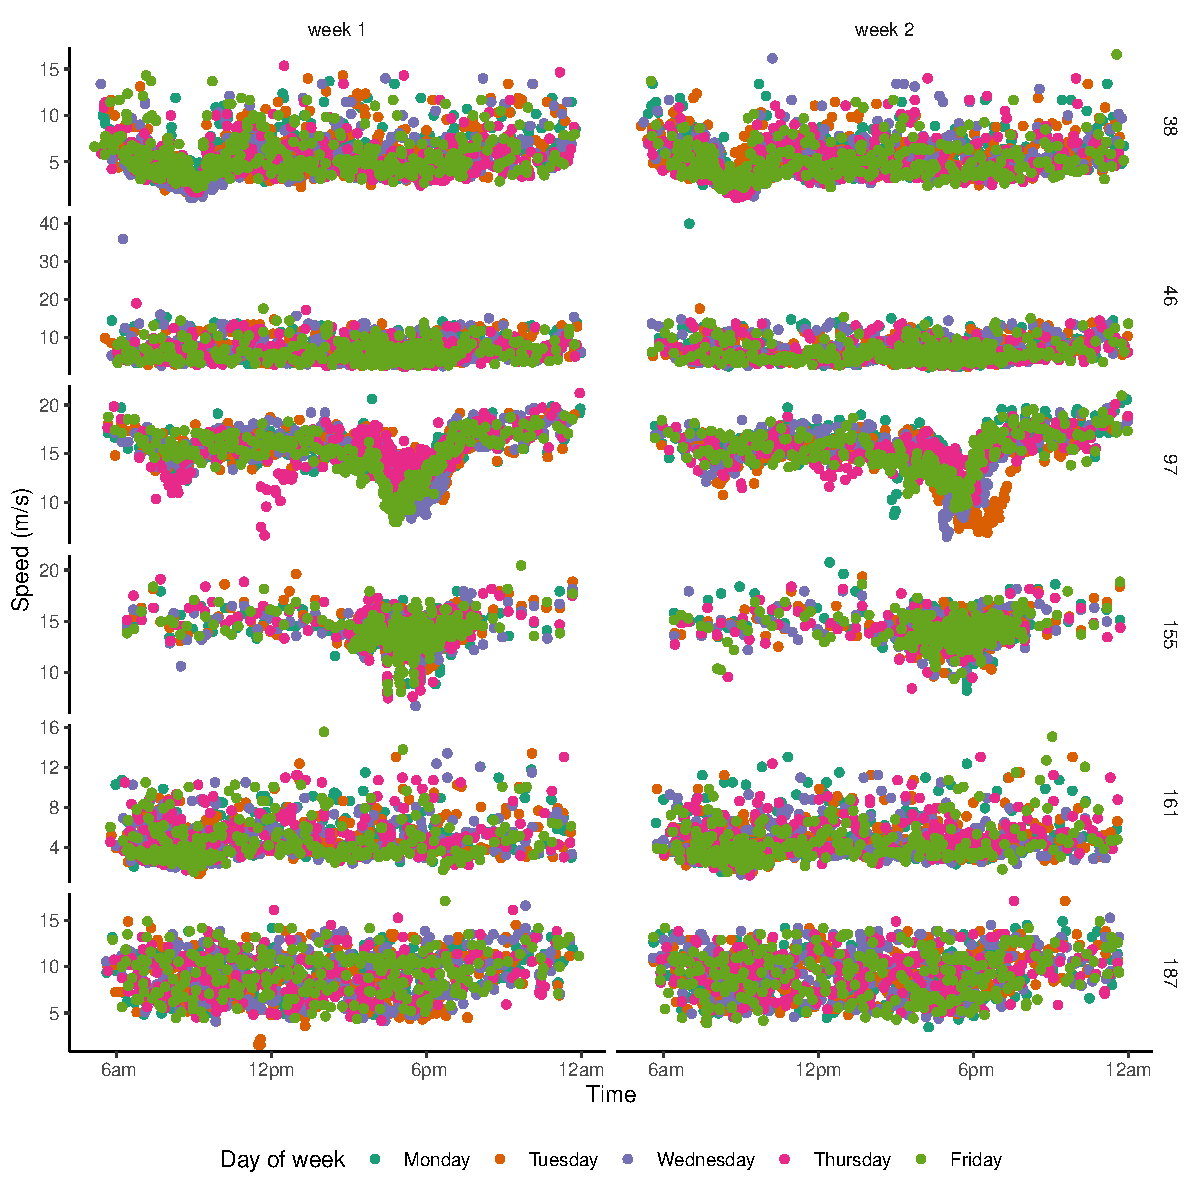
\includegraphics[width=\linewidth]{figure/tt_week1_load-1} 

}

\caption[Vehicle speeds along six roads over of two weeks.]{Vehicle speeds along six roads over the course of two weeks, showing only week days, for training (left) and testing (right).}\label{fig:tt_week1_load}
\end{figure}


\end{knitrout}

\begin{knitrout}\small
\definecolor{shadecolor}{rgb}{0.969, 0.969, 0.969}\color{fgcolor}\begin{figure}

{\centering 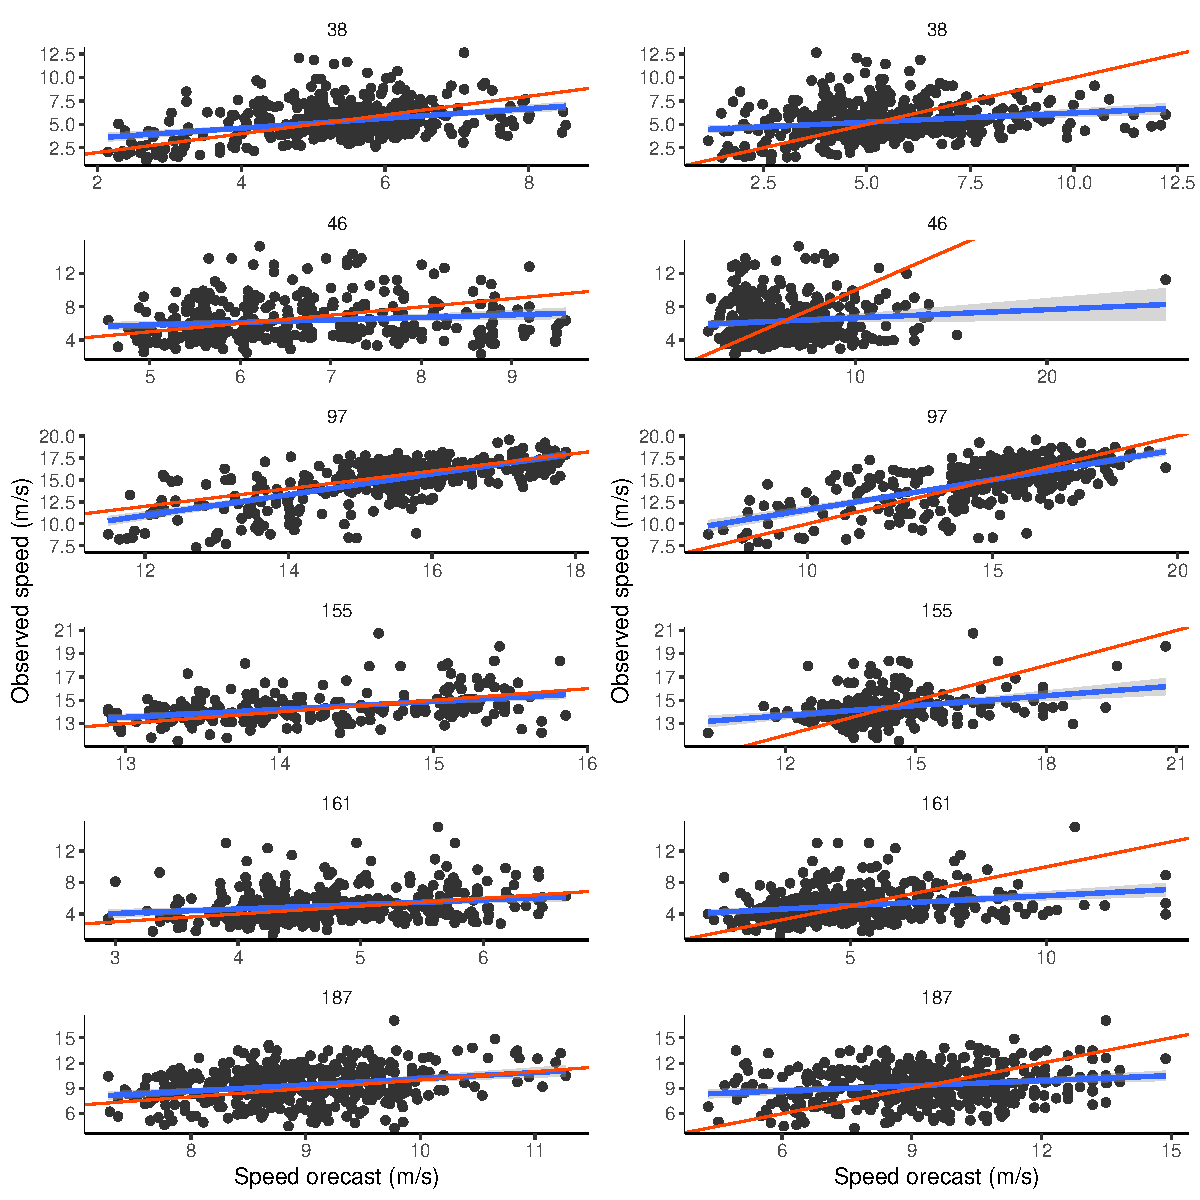
\includegraphics[width=\linewidth]{figure/tt_week1_pred-1} 

}

\caption[Forecasts of average vehicle speeds in 30 minutes versus actual average speed in 30 minutes along segments]{Forecasts of average vehicle speeds in 30 minutes versus actual average speed in 30 minutes along segments. The line of equality (red) indicates a perfect prediction. The closer the best fit line (blue) is to the line of equality, the better the forecasts.}\label{fig:tt_week1_pred}
\end{figure}


\end{knitrout}


Forecasts 30~minutes into the future are shown in \cref{fig:tt_week1_pred} for both the grid-search method, as well as the na\"ive method of using the current average traffic speed as the predictor. The comparative \gls{rmse} values are displayed in \cref{tab:tt_pred_rmse}. However, these are not too different because there is a lot of inherent uncertainty, but demonstrate a slight increase in predictive performance when historical trends are used.


Most importantly, however, is the linear curve (shown in blue in \cref{fig:tt_week1_pred}) compared to the line of equality, in red. The interpretation is that the more accurate the predictions on average, the closer the blue trend line will be to the black line of equality. For our forecast model, we see that in 5 out of 6 segments the two lines are very close, compared to the na\"ive estimate in which case the predictions are often too high or too low.


Further work is needed to improve the forecasting abilities of our model. However, we have designed the framework in such a way that any such improvements can easily be integrated into both the network modelling stage, and the upcoming arrival time prediction stage (see \cref{sec:nw_implementation_forecast} for details).

\begin{table}

\caption{\label{tab:tt_pred_rmse}RMSE results comparing the predictive performance of the two models, in meters per second.}
\centering
\begin{tabular}[t]{lr}
\toprule
Method & RMSE\\
\midrule
Simple & 2.48\\
Forecast & 1.99\\
\bottomrule
\end{tabular}
\end{table}



\section{Particulars of the \rt{} implementation}
\label{sec:nw_implementation}

After stepping through the real-time model, estimation of its parameters, and improvement of forecasts using historical data, the last remaining piece of the network model is its real-time implementation within the \pkg{transitr} package. The first step is, of course, to load the historical data and model the real-time parameters using \prog{JAGS}. These are then inserted into the same database in which we store the \gls{gtfs} and network data.


The network is implemented as independent objects of class \class{Segment}, which are initialised when the program is first started with their model parameter values loaded---if available---from the database. The network state itself is implemented using the \pkg{Eigen} \Cpp{} library, allowing us to store the state vector and uncertainty matrix as an \verb+Eigen::Vector+ or \verb+Eigen::Matrix+, respectively. This library includes all the necessary vector and matrix operations, for example, multiplication. Even though the current state is one-dimensional, we may in future wish to extend this to include, say, the rate of change of speed, which could better model peak periods. This would involve a length-two state vector and $2\times2$ uncertainty matrix. By using \pkg{Eigen}, this change would require minimal code changes. The following sections discuss the initialisation, update, and prediction steps as implemented within \pkg{transitr}.


\subsection{Initialisation}
\label{sec:nw_implementation_init}

The initialisation phase of the network is quite important since in many cases it will be the only piece of information available for speed and arrival time predictions, at least until a vehicle traverses it and provides a real-time observation. Therefore, to initialise a \class{Segment}, we check if there is any historical data available for it: if there is, we set $\NWstate_{\ell,0}$ equal to the historical mean speed of all observations over time. To initialise the uncertainty, we use $\NWstatevar_{\ell 0} = \frac{30}{3.6^2}$~\gls{mps} (which is approximately 30~km/h).

Another part of initialisation is setting the constraint for the \emph{maximum speed}. Since we do not know the speed limit along most road segments, the best we can do is to use the maximum speed limit, 100~km/h, which is approximately 30~m/s. For segments with enough observations, we can use the maximum observed speed to estimate the posted speed limit along the road.



\subsection{State update}
\label{sec:nw_implementation_update}

The state update step is simple due to the segments being independent with one-dimensional states. First, \class{Segment}s are updated after processing the \class{Vehicle}s to collect any new observations (\cref{sec:vehicle_speeds}). Then we perform a parallel iteration over \class{Segment}s: if there are new observations, the update step (\cref{sec:nw_realtime}) is executed. The \pkg{Eigen} library makes this implementation straightforward. Once the state has been updated, the data vector is cleared and the \class{Segment}'s timestamp set to the current time.


\subsection{State forecasts}
\label{sec:nw_implementation_forecast}

While not part of the network state model, forecasting is an essential component of our real-time application. Each \class{Segment} has a \verb+forecast()+ method which returns the forecasted speed given the current timestamp\footnote{This is the time the \class{Segment} was updated, not the wall clock time.} and segment traffic speed. The forecasts are available in 10~minute intervals, so a forecast for 5~minutes uses the current travel time state, while a forecast for 25~minutes uses the 20-minute forecast, and so on, capped at 60~minutes. As for the uncertainty, this comes from the historical data too, but rather than forecasting, we use the historical variance of vehicle speeds at the desired time.

Currently, the forecast method uses the na\"ive constant-speed predictor. Since the arrival time prediction component (\cref{cha:prediction}) accesses forecasts through the \verb+Segment::forecast()+ method, an implementation of the historical-based forecasts\footnote{Or indeed any other desirable forecast method.} will automatically be integrated into the forecast model with no change needed to the prediction component.

